\section{Ứng dụng}
Ngày nay,  các ứng dụng của mô hình tuần tự theo tuần tự đã trở nên rất phổ biến.  Không còn chỉ gói gọn trong các ứng dụng liên quan đến Dịch Máy, mô hình tuần tự theo tuần tự còn được ứng dụng trong các trường hợp sau:
\paragraph{4.1.  Trả lời tự động (Dialog)}
Một trong những ứng dụng thú vị của tuần tự theo tuần tự là Hội Thoại, hay Hệ Thống Trả Lời Tự Động. Đầu vào của Hệ Thống sẽ là yêu cầu hoặc từ phía người dùng F (ví dụ: hỏi "Bạn tên gì"), đầu ra của hệ thống sẽ là phản hồi của hệ thống (E), như trong hàm được giới thiệu dưới đây :
$$\hat{E}=\mathop{argmax}_{\textbf{E}} log P(E|F) - \lambda logP(E)$$
Trong đó,  số hạng thứ nhất $$\mathop{argmax}_{\textbf{E}} log P(E|F)$$ là một hàm giải mã (decoded) thông thường của một mô hình seq2seq trong khi số hạng thứ 2  $$\lambda logP(E)$$ được sử dụng để tăng tính đa đạng của đầu ra,  bằng cách "phạt" những kết quả  đầu ra mà ít tính tương quan với đầu vào E(ví dụ: trả lời: "Tôi không biết").

\paragraph{4.2.  Tóm tắt nội dung tự động (Summarization)}:
Việc tóm tắt nội dung một cách tự động được thực hiện thông qua một số lớp như sau:

\textbf{Rút gọn câu}: Rút gọn và ít làm thay đổi ngữ nghĩa của một câu đơn.

\textbf{Rút gọn một đoạn văn bản}:thực hiện thông qua rút gọn lần lượt các câu trong văn bản.

\textbf{Rút gọn nhiều đoạn văn bản}:thực hiện bằng cách rút gọn nội dung trong nhiều văn bản đơn lẻ thành một văn bản rút gọn duy nhất.

Kỹ thuật này còn được gọi là Tóm tắt nội dung theo phương thức trừu tượng (Abstractive Summarization)

\paragraph{4.3. Tạo diễn giải tự động (Paraphrase Generation)}: Với mô hình diễn giải tự động,  tương ứng với mỗi câu/ngữ cảnh ở đầu vào sẽ cho ra một câu/ngữ cảnh ở đầu ra có cùng ý nghĩa nhưng khác biệt về từ vựng và cú pháp.

\paragraph{4.4. Mô hình hóa các cấu trúc dữ liệu (Model of Structured Data)}: Kỹ thuật seq2seq còn được sử dụng để biến dòng dữ liệu không có cấu trúc (unstructured data) ở đầu vào thành dữ liệu có cấu trúc ở đầu ra theo dạng cây,  dạng bảng hay đồ thị.  Ví dụ sau cho ta thấy điều đó:

\begin{figure}
	\centering
	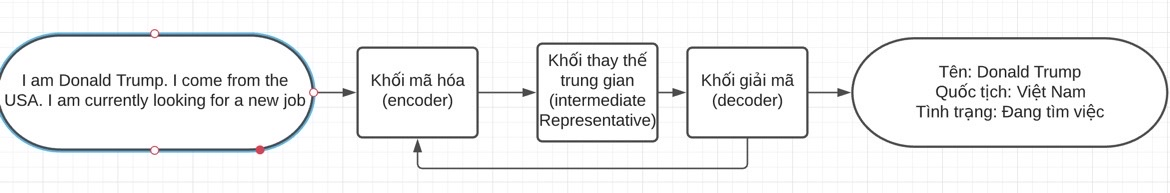
\includegraphics[scale=0.3]{img/structure_data.jpg}
	\caption{Mô hình hóa các cấu trúc dữ liệu}
	\label{structure_data}
\end{figure}